\documentclass{standalone}
\usepackage{pgfplots}

\begin{document}

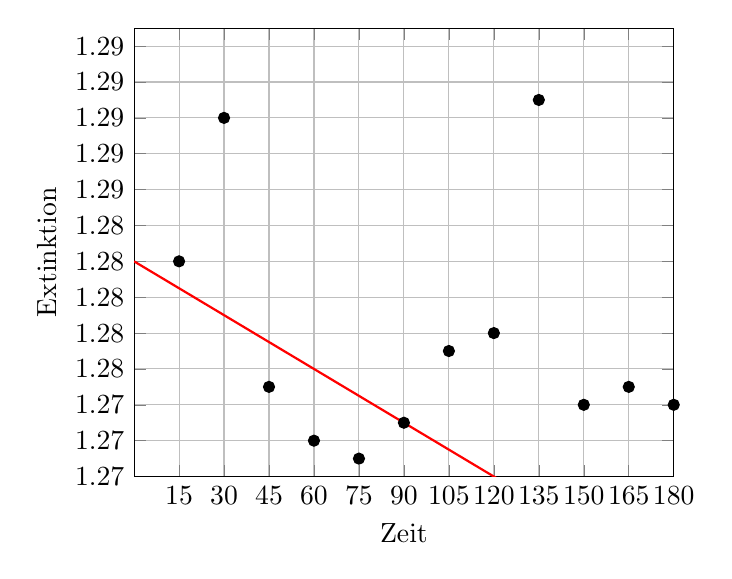
\begin{tikzpicture}
    \begin{axis}[
        xlabel={Zeit},
        ylabel={Extinktion},
        xmin=0, xmax=180,
        ymin=1.27, ymax=1.295,
        xtick={15,30,...,180},
        ytick={1.27,1.272,...,1.295},
        grid=major,
        ]
        % Plot data points
        \addplot[only marks] coordinates {
            (15, 1.282)
            (30, 1.29)
            (45, 1.275)
            (60, 1.272)
            (75, 1.271)
            (90, 1.273)
            (105, 1.277)
            (120, 1.278)
            (135, 1.291)
            (150, 1.274)
            (165, 1.275)
            (180, 1.274)
        };
        
        % Plot trend line
        \addplot[red, thick, domain=0:180, samples=2] {1.282 - 0.0001 * x};
    \end{axis}
\end{tikzpicture}

\end{document}